\documentclass[11pt]{article}
\usepackage[margin = 1in]{geometry}
\usepackage{amsmath}
\usepackage{amssymb}
\usepackage{amsthm} % for proof environment
\usepackage{enumitem}
\usepackage{graphicx}
\usepackage{indentfirst}
\usepackage{caption}
\usepackage{subcaption}
\usepackage{lscape}
\usepackage{multirow}
\usepackage{array}
\usepackage{tikz}
\usetikzlibrary{calc} % for positioning tikz nodes

\renewcommand{\labelenumii}{\alph*)}
\newcommand{\ev}{\mathbb{E}}

%\tikzset{%
%	hollow/.style = {circle,draw,inner sep=1.5},
%	solid/.style = {circle,draw,inner sep=1.5,fill=black}%
%}

\begin{document}

\begin{flushleft}
	Nick Hoffman \\
	Game Theory, Spring 2020 A \\
	Assignment 4 \\
\end{flushleft}

\begin{enumerate}
	\item In the job market signaling model, workers are of type $ \theta\in\{\theta_L, \theta_H\} = \{0.2, 1\} $, each with equal one-half probability. In order to obtain education level $ e $ as a signal to the firms, the workers pay cost $ e/\theta $. The firm sets its wages such that $ w(e) = \ev(\theta|e) $. Thus, a worker of type $\theta$ receives utility $ w(e) - \frac{e}{\theta} $. The firms form beliefs of the type $ \mu(\theta|e) $, the probability that the worker is of type $\theta$ given her level of education. 
	\begin{enumerate}
		\item In a separating equilibrium, workers of each type choose different levels of education $ e^* $, where $ e^*(\theta_L) < e^*(\theta_H) $. For simplicity, I denote these equilibrium levels of education $ e_L $ and $ e_H $, respectively. The firms, knowing this, can differentiate, and thus for the low worker, they set
		\[w(e_L) = \ev(\theta_L|e_L) = \mu(e_L)\theta_L + \big(1 - \mu(e_l)\theta_H\big) = \theta_L\]
		The low-type worker then solves
		\[\max_e \theta_L - \frac{e_L}{0.2}\] 
		and thus chooses $ e_L = 0 $. 
		
		The firm can set a range of wage schedules $ w(e) $ to support a range of education levels for the high type. As with the low type, the firm will set $ w(e_H) = \theta_H = 1 $. What remains to be determined is the level of education at or above which a worker can earn the wage of 1. To show the result visually, Figure \ref{fig1} plots indifference curves for the high and low types:
		
		\begin{figure}[!htbp]
			\centering
			\caption{Separating Equilibrium}
			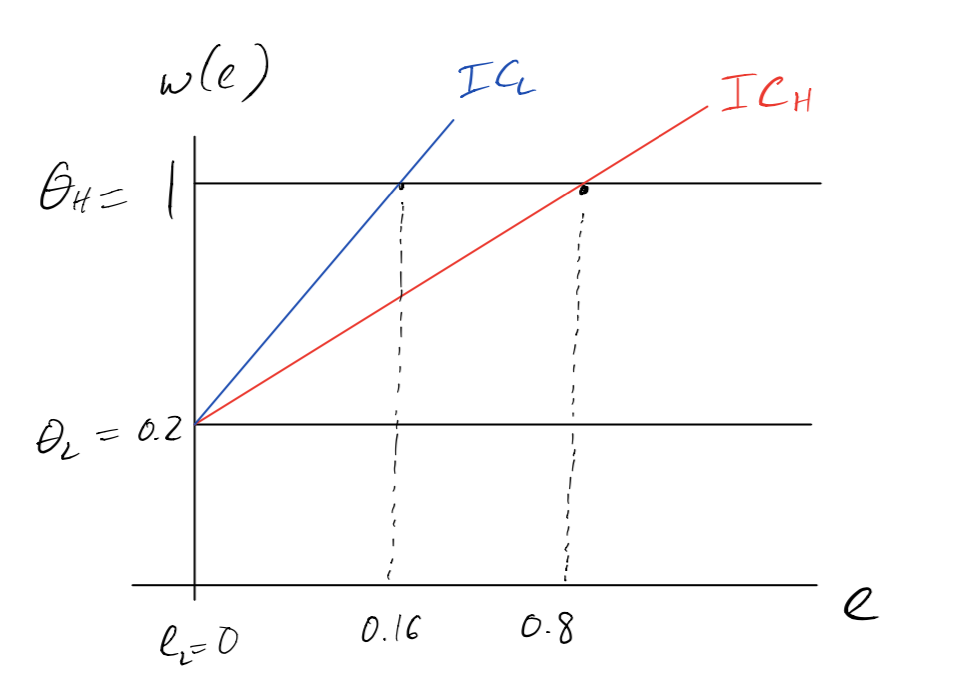
\includegraphics[scale=0.6]{fig_1_separating}
			\label{fig1}
		\end{figure}
		The red line shows the indifference curve for a worker of type $\theta_H$, and the blue for type $\theta_L$. The intersections of these indifference curves with the line at $\theta_H$ give bounds on the levels of education for the high type that can be supported in a separating equilibrium.
		
		The firm can sustain any level of education for the high type $ e_H\in[0.16, 0.8] $ by offering $ w(e) = 1 $ for any level of education $ e\in[e_H, \infty] $. If they attempt to sustain $ e_H < 0.16 $, then the high-type workers are better off getting zero education. If the firm attempts to sustain $ e_H > 0.8 $, meanwhile, the low-type workers will also choose $ e_H $, and thus this level cannot be a separating equilibrium. Thus, the  equilibrium which sustains $ e_L = 0 $ and $ e_H = \hat{e} $ is characterized by firm beliefs
		\[\mu(\theta_H|e) = \begin{cases}
		0 & e\in[0, \hat{e}) \\ 
		1 & e\in[\hat{e}, \infty)
		\end{cases}\]
		and wage schedule 
		\[w(e) = \begin{cases}
		0.2 & e\in[0, \hat{e}) \\ 
		1 & e\in[\hat{e}, \infty)
		\end{cases}\]
		
		\item In the pooling equilibrium, both types of workers choose the same level of education, the firm sets one wage, equal to the unconditional expectation of $\theta$:
		\[w(e) = 0.5\theta_L + 0.5\theta_H = 0.6 \]
		Figure \ref{fig2} shows this wage along with indifference curves for the high and low type workers:
		
		\begin{figure}[!htbp]
			\centering
			\caption{Pooling Equilibrium}
			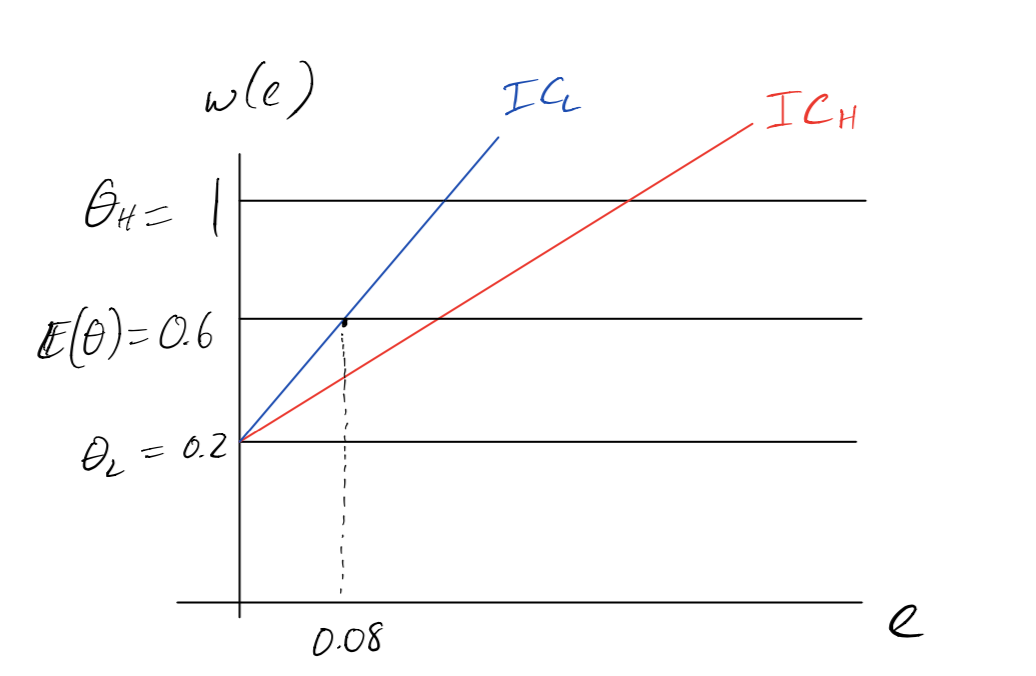
\includegraphics[scale=0.6]{fig_2_pooling}
			\label{fig2}
		\end{figure}
		Here, the intersection of the blue indifference curve ($\theta_L$) and the line at $ \ev(\theta) = 0.6 $ is the maximum level of education that can be sustained in a pooling equilibrium.
		
		The firm can sustain any pooling equilibrium level of education $ \hat{e}\in[0, 0.08] $. If they set $ \hat{e} > 0.08 $, the low-type workers are better off choosing $ e_L = 0 $. The pooling equilibrium that sustains $ \hat{e}\in[0, 0.08] $ is fully characterized by firm beliefs
		\[\mu(e) = \begin{cases}
		0 & e\in[0, \hat{e}) \\ 
		\frac{1}{2} & e\in[\hat{e}, \infty)
		\end{cases}\]
		and wage schedule
		\[w(e) = \begin{cases}
		0.2 & e\in[0, \hat{e}) \\ 
		0.6 & e\in[\hat{e}, \infty)
		\end{cases}\]
	\end{enumerate} \newpage

	\item The tree for the extensive form of the game is as follows:
	
	\begin{figure}[!h]
		\centering
		\caption{Game Tree}
		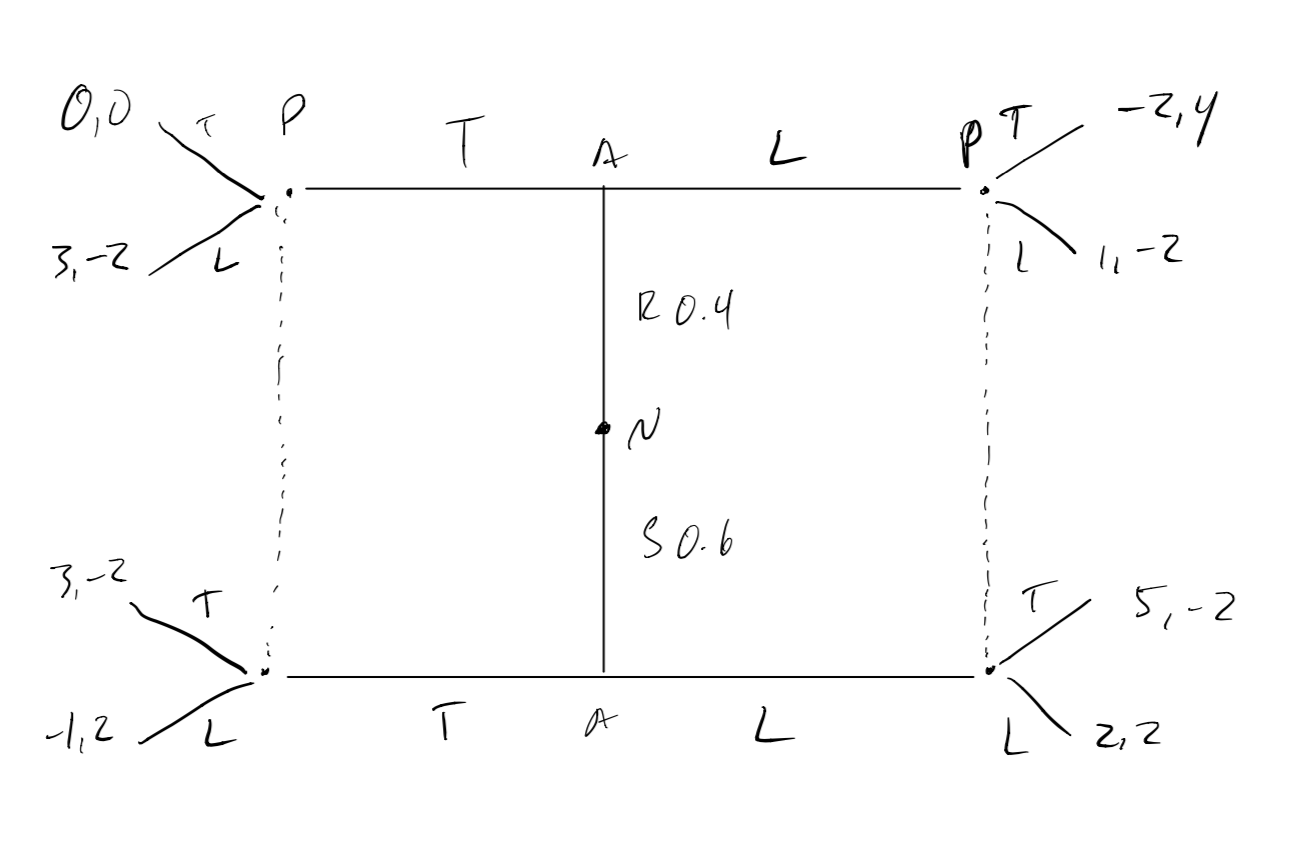
\includegraphics[scale=0.6]{fig_3_tree}
		\label{fig3}
	\end{figure}


	There are no separating or pooling Perfect Bayesian equilibria in pure strategies. In order to find the mixed-strategy PBE, I define variables for the players' respective strategies. Let $ T_R $ and $ L_R $ denote Anna's actions, respectively, of taking and leaving her umbrella when it rains, and $ T_S $ and $ L_S $ the actions of taking and leaving when it is sunny. Anna's corresponding mixed strategies are $ \gamma_R $ and $\gamma_S$, indicating the probability of her taking her umbrella when it rains and is sunny, respectively. Note that because he cannot observe the weather forecast, Paul observes either $ (T_R, T_S) $ or $ (L_R, L_S) $. To differentiate nodes, let $ x_1 $ represent the node at which  Anna chooses upon observing a forecast of rain, and $ x_2 $ the node at which she chooses upon observing sun. Let $ \delta $ be the probability that Paul takes his umbrella given that he observes Anna leave hers, and $ \eta $ be the probability that he takes his umbrella given that Anna has taken hers. Finally, let $\alpha$ be the probability that Paul assigns to it raining when he observes $ L $, and $\beta$ be the probability that he assigns to it raining when he observes $ T $. The following diagram illustrates these new variables: \newpage
	
	\begin{figure}[!h]
		\centering
		\caption{Game Tree, with Additional Detail}
		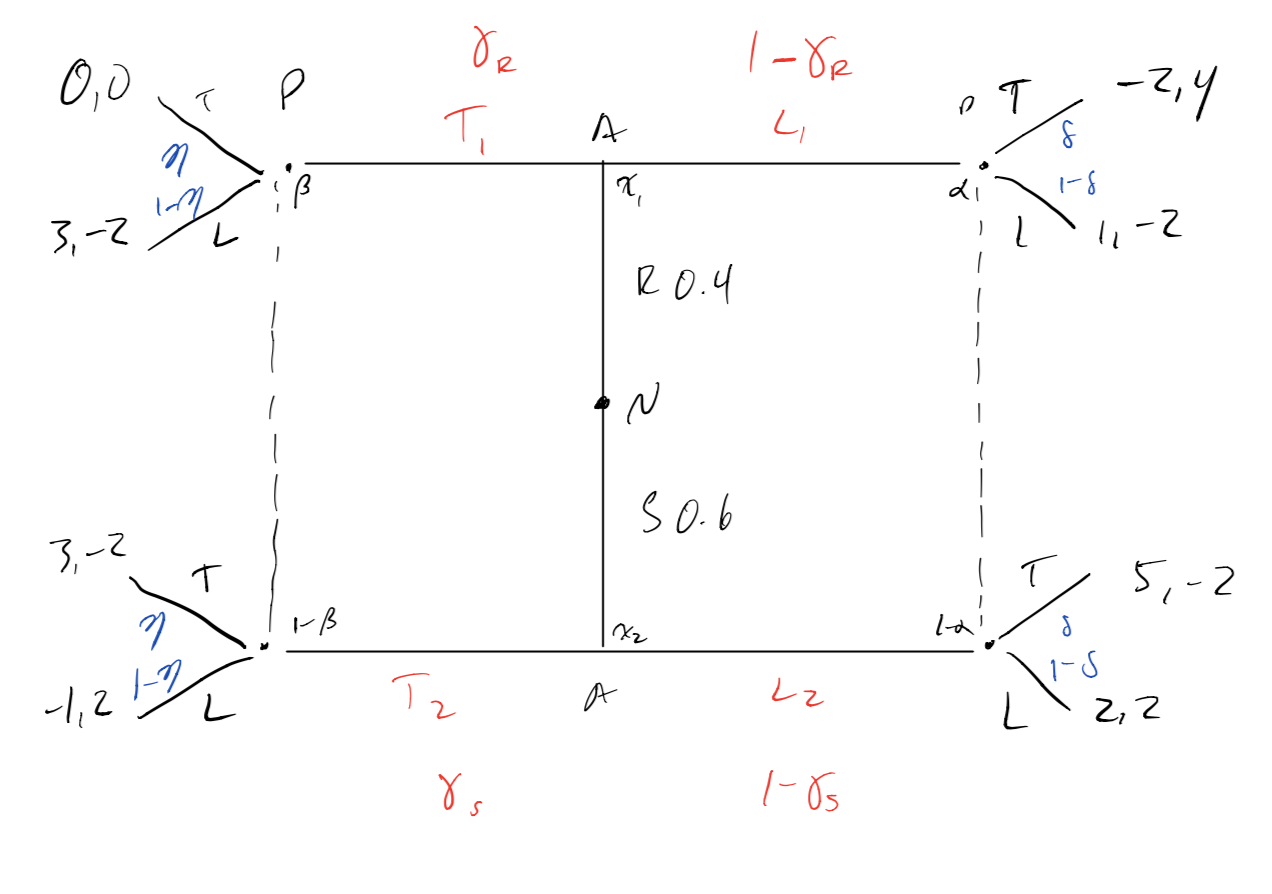
\includegraphics[scale=0.6]{fig_4_tree_color}
		\label{fig4}
	\end{figure}
	
	Paul's utilities from responding to Anna's actions are as follows:
	\begin{align*}
	\text{Observe L: }\quad &U(T) = 6\alpha - 2 \\
	& U(L) = 2 - 4\alpha \\
	\text{Observe T: } \quad &U(T) = 2\beta - 2 \\
	&U(L) = 2 - 4\beta
	\end{align*}
	Thus, his best responses are as follows: 
	\[BR(\alpha) = \begin{cases}
	T & \alpha > \frac{2}{5} \\
	[T,L] & \alpha = \frac{2}{5} \\
	L & \alpha < \frac{2}{5} \\
	\end{cases} \]%
	\[BR(\beta) = \begin{cases}
	T & \beta > \frac{2}{3} \\
	[T,L] & \beta = \frac{2}{3} \\
	L & \beta < \frac{2}{3} \\
	\end{cases} \]
	
	To begin, note that $ \gamma_R = \gamma_S = 1 $ cannot be an equilibrium: in this case, Paul updates his beliefs in the following way: 
	\[\beta = \frac{0.4\gamma_R}{0.4\gamma_R + 0.6\gamma_S} = 0.4\]
	By the above, Paul plays $ L $. $\alpha$, then, must be $ 2/5 $, otherwise, these would be pure strategies, which do not constitute an equilibrium in this case. Here, however, there is no value for $\delta$ such that Amy is still better off playing $ (T_1, T_2) $. Thus, this cannot be an equilibrium.
	
	If Anna plays $ \gamma_R  = \gamma_S = 0 $, then Paul will update his beliefs in the following way:
	\[\alpha = \frac{0.4}{0.4 + 0.6} = 0.4 = \frac{2}{5}\]
	and thus he will randomize between $ T $ and $ L $. As before, $\beta$ must be $ 2/3 $, otherwise this would not be an equilibrium. To determine Paul's strategy, note that Anna's best responses at nodes $ x_1 $ and $ x_2 $ are:
	\begin{align*}
	x_1: \quad & U(T_1) = 3 - 3\eta \\
	&U(L_1) = 1 - 3\delta \\
	x_2:\quad & U(T_2) = 4\eta - 1 \\
	& U(L_1) = 3\delta + 2
	\end{align*}
	Thus, Anna will be better off playing $ (L_1, L_2) $ if Paul sets his strategy such that, given $\eta$, 
	\[\delta\in\left[\frac{3}{4}\eta - \frac{3}{4}, \eta - \frac{2}{3}\right]\]
	Thus, the Perfect Bayesian Equilibrium is as follows: 
	\begin{itemize}
		\item $ P_1 $: $ \gamma_R = \gamma_S = 0 $ $ (L_1, L_2) $
		\item \[P_2: \begin{cases}
		\eta T \oplus (1 - \eta)L & \text{if $ (T_1, T_2) $} \\
		\delta T \oplus (1 - \delta) L & \text{if $ (L_1, L_2) $}
		\end{cases}\]
		where 
		\[\delta\in\left[\frac{3}{4}\eta - \frac{3}{4}, \eta - \frac{2}{3}\right]\]
		\item Beliefs: $\alpha = 2/5$, $ \beta = 2/5 $ 
	\end{itemize}

	Note that this is the only PBE: if we consider $ \gamma_R\in(0,1) $ and $ \gamma_S\in(0,1) $, these proportions Will affect Paul's beliefs $\alpha$ and $\beta$. Here there are four cases:
	\begin{enumerate}[label = (\arabic*)]
		\item $\alpha\neq 2/5$, $\beta\neq 2/3$ This case is not an equilibrium, as it would induce Paul to play pure strategies at both information sets--as mentioned above, no such equilibrium exists. 
		\item $\alpha = 2/5$, $\beta = 2/3$ This would require $\gamma_R$ and $\gamma_S$ to be such that 
		\begin{align*}
		\frac{0.4\gamma_R}{0.4\gamma_R + 0.6 \gamma_S} &= \frac{2}{3} \\
		\frac{0.4(1 - \gamma_R)}{0.4(1 - \gamma_R) + 0.6 (1 - \gamma_S)} &= \frac{2}{5}
		\end{align*}
		There is no combination of $ \gamma_R\in(0,1) $ and $ \gamma_S\in(0,1) $ that satisfies both equations. 
		\item $ \alpha \neq 2/5 $, $ \beta = 2/3 $. In this case, 
		\[\frac{0.4\gamma_R}{0.4\gamma_R + 0.6 \gamma_S} = \frac{2}{3}\]
		and thus $ \gamma_R = 2\gamma_S $, which implies $ \alpha < 2/5 $, and thus Paul plays $ L $ when he observes $ L $. Given this strategy, however, there is no randomization that Paul can play upon observing $ T $ that makes Anna indifferent at both $ x_1 $ and $ x_2 $, and thus this cannot be an equilibrium.
		\item $ \alpha = 2/5 $, $ \beta \neq 2/3 $. In this case, 
		\[\frac{0.4(1 - \gamma_R)}{0.4(1 - \gamma_R) + 0.6 (1 - \gamma_S)} = \frac{2}{5}\]
		and thus $ \gamma_R = \gamma_S $, and so $\beta = 0.4$, and thus Paul plays $ T $ when he observes $ T $. However, there is no mixed strategy that Paul can play upon observing $ L $ such that Anna is still indifferent between the two, and thus this cannot be an equilibrium.
	\end{enumerate}
	Thus, the PBE described above is unique. 
	
	\item \begin{enumerate}
		\item This game has two Perfect Bayesian equilibria:
		\begin{enumerate}[label = \roman*.]
			\item Strategies:
			\begin{gather*}
			P_1: \delta = 0 (R) \\
			P_2: \beta = 0 (C) \\
			P_3: \alpha = 1 (L)
			\end{gather*}
			Beliefs:
			\begin{gather*}
			P_2: \gamma = 0 \\
			P_3: \mu = 0
			\end{gather*}
			
			\item Strategies:
			\begin{gather*}
			P_1: \delta = 0 (R) \\
			P_2: \beta = 1 (S) \\
			P_3: \alpha = 0 (R)
			\end{gather*}
			Beliefs:
			\begin{align*}
			P_2: \gamma &= 0 \\
			P_3: \mu &= \text{any beliefs}
			\end{align*}
		\end{enumerate}
	
		\item Of the two equilibria above, only the first is a sequential equilibria. To show this, consider the second strategy, where player 2 plays $ S $. Suppose that instead of playing $ S $ with probability one, player 2 ``trembles'', and plays $ C $ with probability $ \varepsilon^n $, such that $ \varepsilon^n\to 0 $. This allows us to specify player 3's beliefs about $\mu$, the conditional probability of being on the left side given that play reaches his turn. His belief is given by
		\[\mu = \frac{(1 - \delta)\varepsilon^n}{\varepsilon^n} = (1 - \delta)\]
		However, given that this is player 2's belief, it is optimal for him to play $ R $ if given the chance, as his expected payoffs are:
		\[u_3(R) = \delta,\quad u_3(L) = 1 - \delta \]
		In either case, R is a dominating strategy for player 1, and thus all players know that $\delta = 0$. Thus, while the second equilibrium above is a PBE, it is not a sequential PBE, as player 3's actions are not sequentially rational. 
		
		The first equilibrium, meanwhile, is sequentially rational. As above, player 3's conditional beliefs can be found using Bayes' Rule, in particular,
		\[\mu = \frac{\delta (1 - \beta)}{1 - \beta} = \delta\]
		Similarly, player 2 forms the belief $ \gamma = \delta $. Knowing this, player 3 will play $ R $, $\alpha = 1$. Player 2's payoffs, then, are as follows:
		\[u_2(S) = 1 - \delta, \quad u_2(C) = 2\alpha(1 - \delta)\]
		Because $\delta = 0$ and $\alpha = 1$, player 2 is better off playing $ C $, $\beta = 0$. Thus, at each information set in the first equilibrium, the players play sequentially rational strategies, and thus this is the sequential equilibrium. 
	\end{enumerate}
\end{enumerate}

\end{document}